
\documentclass[notes=show]{beamer}
%%%%%%%%%%%%%%%%%%%%%%%%%%%%%%%%%%%%%%%%%%%%%%%%%%%%%%%%%%%%%%%%%%%%%%%%%%%%%%%%%%%%%%%%%%%%%%%%%%%%%%%%%%%%%%%%%%%%%%%%%%%%%%%%%%%%%%%%%%%%%%%%%%%%%%%%%%%%%%%%%%%%%%%%%%%%%%%%%%%%%%%%%%%%%%%%%%%%%%%%%%%%%%%%%%%%%%%%%%%%%%%%%%%%%%%%%%%%%%%%%%%%%%%%%%%%
\usepackage{mathpazo}
\usepackage{hyperref}
\usepackage{multimedia}
\usepackage[spanish,activeacute]{babel}
\usepackage{color}
\setbeamercovered{dynamic}
%TCIDATA{OutputFilter=LATEX.DLL}
%TCIDATA{Version=5.50.0.2890}
%TCIDATA{<META NAME="SaveForMode" CONTENT="1">}
%TCIDATA{BibliographyScheme=Manual}
%TCIDATA{Created=Thursday, June 14, 2007 23:33:38}
%TCIDATA{LastRevised=Friday, June 15, 2007 01:42:35}
%TCIDATA{<META NAME="GraphicsSave" CONTENT="32">}
%TCIDATA{<META NAME="DocumentShell" CONTENT="Other Documents\SW\Slides - Beamer">}
%TCIDATA{CSTFile=beamer.cst}

%\newtheorem{theorem}{Teorema}[section]
\newtheorem{claim}{Caracter\'isticas}[section]
\newenvironment{stepenumerate}{\begin{enumerate}[<+->]}{\end{enumerate}}
\newenvironment{stepitemize}{\begin{itemize}[<+->]}{\end{itemize} }
\newenvironment{stepenumeratewithalert}{\begin{enumerate}[<+-| alert@+>]}{\end{enumerate}}
\newenvironment{stepitemizewithalert}{\begin{itemize}[<+-| alert@+>]}{\end{itemize} }
\usetheme{CambridgeUS}
\input{tcilatex}
\begin{document}

\title[Crecimiento y decrecimiento de pol\'igonos]{Crecimiento y
decrecimiento de pol\'igonos mediante paralelas}
\author[Jhones]{Nelson Gonz\'alez Jhones}
\institute[Matcom UH]{Universidad de la Habana\\
Facultad de Matem\'atica y Computaci\'on}
\date[06/07]{Junio 2007}
\maketitle

\section{Descripci\'{o}n del problema}

\subsection{Caracter\'isticas}

\begin{frame}
\frametitle{Descripci\'{o}n del problema}

\begin{columns}[6cm]

\column{7cm}

%\begin{claim}
\begin{block}{Caracter\'isticas}
\begin{enumerate}
\item<1-| alert@1> \textnormal{\small{El resultado consiste en un conjunto de pol\'igonos $P'$.}}
\item<2-| alert@2>  \textnormal{\small{A cada segmento en $P'$ le corresponde un \'unico segmento en el pol\'igono original $P$.}}
\item<3-| alert@3> \textnormal{\small{Sean los segmentos $s$ y $s'$ tal que $s \in P$ y $s' \in P'$}. Si $s$ es el segmento correspondiente de $s'$ entonces $s'$ es paralelo a $s$ y la distancia entre ellos es $d$. }
\qedhere

%
\end{enumerate}
\end{block}


%\end{claim}

\column{5cm}

\begin{figure}[htbp]
	\centering
		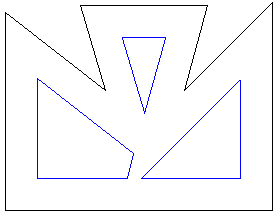
\includegraphics[width = 4cm, height=4cm]{C:/c/conjunto.png}
	\label{fig:corte1}
\end{figure}


\end{columns}
\transdissolve<2,3>[duration=0.4]
\end{frame}

\section{Una forma de abordar el problema}
\subsection{Una forma de abordar el problema}

\begin{frame}
\frametitle{Una forma de abordar el problema}
\begin{block}{}
\begin{enumerate}

	\item<1-| alert@1> Trazar un paralela a cada segmento de $P$ a distancia $d$.
	\item<2-| alert@2> Consecuencias no deseables.
	\item<3-| alert@3> M\'ultiples intersecciones.
	\item<4-| alert@4> Poligonal resultante no simple.
	\item<5-| alert@5> Regiones no deseables.
	\item<6-| alert@6> Eficiente para distancias suficientemente peque\~nas.
	\end{enumerate}	
\end{block}
\transboxout<2,3,4,5,6>[duration=0.4]
\end{frame}

\begin{frame}
\frametitle{Algunos ejemplos}

\begin{columns}[5cm]
\column{5cm}

\begin{figure}
	\centering
		\includegraphics<1>[width = 4cm, height=4cm]{C:/c/zapato.png}	
		\caption{Consecuencias no deseables}
\end{figure}


\column{5cm}

\begin{figure}
	\centering
		\includegraphics<1>[width = 3.5cm, height=4cm]{C:/c/tony.png}	
		\caption{Poligonal resultante no simple}
\end{figure}


\end{columns}

\end{frame}
\subsection{La idea del Plane-Sweep}
\begin{frame}
\frametitle{Plane Sweep}
\begin{enumerate}
	\item<1-| alert@1>Detecci\'on de las regiones.
	\item<2-| alert@2>Clasificaci\'on en deseables o no.  
	\item<3-| alert@3>Regiones inducidas por intersecciones.	
\end{enumerate}
\transboxin[duration=0.3]
\end{frame}
%%%%%%%%%%%%%%%%%%%%%%%%%%%%%%%%%%%%%%
\begin{frame}
<1>[label=pspacecomplete2] 
\frametitle{Soporte}

\begin{block}{Lema}
\footnotesize{Sean $r_{1}$ y $r_2$ dos rayos que van desde los puntos $x_1$ y $x_2$ respectivamente, hasta el infinito. Si $x_1$ y $x_2$ pertenecen a una misma regi\'on determinada por $C$, entonces la diferencia entre los cortes de izquierda a derecha y los cortes de derecha a izquierda de $C$ con $r_1$ y $r_2$ ser\'a la misma.}\end{block}

\begin{overprint}
\onslide<1>
\hyperlink{pspacecomplete2<2>}{\beamergotobutton{Detalles de la demostraci\'on}}

\onslide<2> 

\begin{proof}
\footnotesize{ Sea $z$ una curva orientada que pase por los puntos $x_1$ y $x_2$. Sup\'ongase que se realizan dos recorridos sobre $z$ a partir de los puntos $x_1$ y $x_2$ en sentidos contrarios. Sean $d_1$ y $i_1$ los cortes de derecha a izquierda y los cortes de izquierda a derecha respectivamente, de $z$ con $C$ en el recorrido a partir de $x_1$. As\'i mismo, $d_2$ y $i_2$ representan los cortes del recorrido a partir de $x_2$. Sup\'ongase adem\'as, que entre $x_1$ y $x_2$, $z$ no corta a $C$. Entonces se cumple que $d_1 + i_2 = d_2 + i_1$ ya que $C$ es cerrada y por tanto $d_1 - i_1 = d_2 - i_2$. \newline

En particular, los recorridos a partir de $x_1$ y $x_2$ pueden ser rectos y con esto queda terminada la demostraci\'on.}
\end{proof}

\only<beamer>{\hfill\hyperlink{pspacecomplete2<1>}{\beamerreturnbutton{Regresar}}}
\end{overprint}
\transdissolve[duration=0.4]
\end{frame}
%%%%%%%%%%%%%%%%%%%%%%%%%%%%%%%%%%%%%%%%%%%%%%%%%
\subsection{\textquestiondown Criterios o conjeturas?}
\begin{frame}
\frametitle{Regiones inexistentes}

\begin{columns}[6cm]
\column{7cm}


\begin{block}{Definici\'on}
Se entender\'a por \emph{\alert{segmento invertido}} de $P'$ aquel cuyo sentido se encuentra en oposici\'on con su correspondiente en $P$.
\end{block}

 \textcolor{violet}{\newline Nota:} Sentido en contra de las manecillas del reloj.%

\column{5cm}

\begin{figure}[htbp]
	\centering
		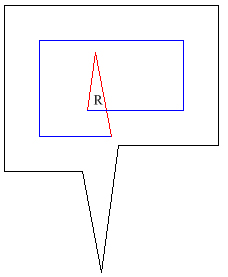
\includegraphics[width = 3.5cm, height=4cm]{C:/c/pico1.png}
\end{figure}

\end{columns}
\transsplithorizontalin[duration=0.4]
\end{frame}
%%%%%%%%%%%%%%%%%%%%%%%%%%%%%%%%%%%%%%%%%%%%%%%%%%%%%%%%%%%%%%%%%%%%%%%%%%%%
\begin{frame}
\frametitle{\textquestiondown Criterios o conjeturas?}

\begin{block}{Criterio}
\footnotesize{Si en el resultado se encuentra una cadena de segmentos invertidos de
longitud mayor que dos, entonces son eliminados todos los segmentos de la cadena
excepto el primero y \'{u}ltimo. }
\end{block}
\pause
\begin{block}{Criterio}
\footnotesize{Si se tiene un segmento invertido aislado, significa que, a la distancia dada, ese
segmento no debe verse reflejado en el resultado. En consecuencia de esto, es
eliminado y es hallada la intersecci\'{o}n (si existe) entre los segmentos
adyacentes a este. }\end{block}
\pause
\begin{block}{Criterio}
\footnotesize{Teniendo un par de segmentos invertidos, no eliminar aquel que luego de la
eliminaci\'{o}n de su adyacente invertido deje de serlo. En caso de que esto
sea imposible ambos son eliminados, por otra parte en el caso de tener
reflexividad no se lleg\'o a contar con un criterio s\'{o}%
lido sobre cual, de los dos segmentos, debiera eliminarse.}\end{block}

\transboxout<1>[duration=0.1]
\transboxin<2>[duration=0.4]
\transboxout<3>[duration=0.4]
\end{frame}

\begin{frame}
\frametitle{Nuevas regiones inexistentes}

\begin{block}{Segundo Criterio}
Teniendo un par de segmentos $s_1$ y $s_2$ consecutivos en $P'$, que no lo son en $P$. Si $s_1$ est\'a a la izquierda (a la derecha) de $s_2$ en $P'$ y $s_1$ se encuentra a la derecha (a la izquierda) de $s_2$ en $P$ entonces $s_1$ es considerado como invertido por este criterio. De forma an\'aloga es analizada la posici\'on de $s_2$ respecto a $s_1$.
\end{block}

\transdissolve[duration=0.4]
\end{frame}

\begin{frame}
\frametitle{Segundo Criterio}

\begin{figure}
	\centering
		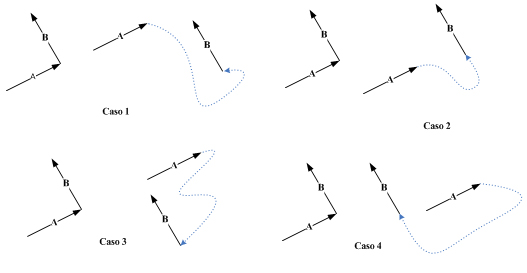
\includegraphics[width = 10cm, height=4cm]{C:/c/casos1.png}	
		\caption{En el \textbf{Caso 1} B est\'a invertido , en el \textbf{Caso 2} ninguno de los dos est\'an invertidos, en el \textbf{Caso 3} ambos est\'an invertidos y en el \textbf{Caso 4} A est\'a invertido. }
\end{figure}
\transboxout[duration=0.4]
%\transdissolve[duration=0.4]uuyuy
\end{frame}
\subsection{Conclusiones}


\begin{frame}
\frametitle{Resultados}

\begin{block}{}
\begin{itemize}
	\item<1-| alert@+>La eliminaci\'on local provoca la eliminaci\'on de segmentos que deberian aparecer en el resultado
	\item<2-| alert@+>Eficiente para distancias peque\~nas.
	\item<3-| alert@+>Intersecciones con la original parcial y completamente.  
\end{itemize}
\end{block}

\transsplitverticalout[duration=0.4]
\end{frame}

\begin{frame}
\frametitle{Ejemplos}
\begin{figure}
	\centering
		\includegraphics<1>[height=3cm, width=10cm]{C:/c/comp2.png}%j		
		\includegraphics<2>[height=3cm, width=7cm]{C:/c/parcial.png}%j	 	
		\caption{\only<1>{(a) Resultado directo de hacer la paralela a cada segmento, (b) resultado de la eliminaci\'on de las regiones no deseables y (c) resultado de la especificaci\'on. }\only<2>{Corte parcial con el pol\'igono original}}
\end{figure}
\end{frame}
%%%%%%%%%%%%%%%%%%%%%%%%%%%%%%%%%%%%%%%%%%%%%%%%%%%%%%%   

\section{El esqueleto recto}

\subsection{\textquestiondown Qu\'e es el esqueleto recto?}

\begin{frame}
\frametitle{Esqueleto recto}
\framesubtitle{\textquestiondown Qu\'e es el esqueleto recto?	}
\begin{block}{}
Un esqueleto recto sobre un grafo plano $G$ es una partici\'on del plano en regiones de forma tal que, cada regi\'on refleja, de manera apropiada, la forma geom\'etrica de $G$.
\end{block}
\pause
\begin{block}{Definici\'on}
El \alert{esqueleto recto}, de un pol\'igono simple en el plano, queda definido por el rastro que
dejan los v\'ertices del pol\'igono inicial cuando este se ve encogido o ensanchado, movi\'endose
de cada una de sus aristas a una misma velocidad.
\end{block}
\transdissolve<2>[duration=0.4]
\end{frame}

\begin{frame}
\frametitle{Ejemplo}
\begin{figure}[htbp]
	\centering
		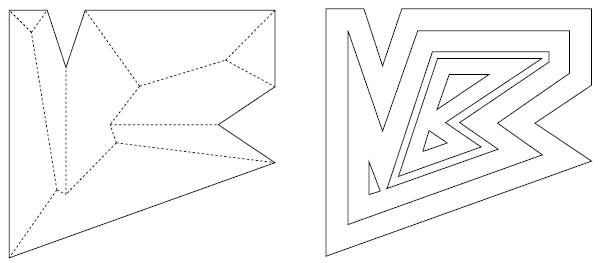
\includegraphics[width=10cm, height=4.5cm]{../../../../../c/esq2.png}%n
	\caption{Esqueleto recto y jerarqu\'ia de pol\'igonos.}
\end{figure}
\transboxin[duration=0.4]
\end{frame}

\begin{frame}
\frametitle{Eventos}
	\begin{enumerate}
		\item<1-> \emph{\alert{Evento de arista}}: La longitud de una arista se reduce a
cero, la arista se desvanece.
		\item<2-> \emph{\alert{Evento de divisi\'on}}: Una arista es dividida, un v\'{e}%
rtice reflexivo se mueve hacia esta arista dividiendo el pol\'{\i}gono entero.
	\end{enumerate}%| alert@2
	\transsplitverticalout<2>[duration=0.5]
\end{frame}

\begin{frame}
\end{frame}

\subsection{Propiedades b\'asicas}

%%%%%%%%%%%%%%%%%%%%%%%%%%%%%%%%%%%%%%%%%%%%%%%%%%%%%%
\begin{frame}
\frametitle{Preliminares}

\begin{block}{Definici\'on}
\alert{V\'{e}rtice reflexivo} de un pol\'igono: v\'{e}rtice cuyas aristas incidentes forman un \'{a}ngulo mayor que $\pi$ en el interior del \ pol\'{\i}gono. V\'ertice convexo: v\'ertice que no es reflexivo.					
\end{block}
\pause
\begin{block}{Definici\'on}
\alert{Arco reflexivo} arco que contiene, en la frontera de la cu\~na en la que \'el se encuentra, a ambas aristas que definen dicha cu\~na.					
\end{block}
\transsplitverticalin<1>[duration=0.5]
\transsplitverticalout<2>[duration=0.5]
\end{frame}


\begin{frame}
<1>[label=pspacecomplete] 
\frametitle{Propiedades b\'asicas}

\begin{block}{Lema}
$S(P)$ es un \'{a}rbol y consiste en exactamente $n$ caras conectadas, $n-2$
nodos y $2n-3$ arcos.
\end{block}

\begin{overprint}
\onslide<1>
\hyperlink{pspacecomplete<2>}{\beamergotobutton{Detalles de la demostraci\'on}}

\onslide<2> 

\begin{proof}
 La construcci\'{o}n de una cara $f(e)$ comienza en su arista, $e$, de $P$. $%
f(e)$ no puede ser dividida a\'{u}n cuando $e$ parezca serlo. La construcci%
\'{o}n de $f(e)$ est\'{a} completa cuando (cada parte de) $e$ ha sido
reducida a cero. Como $e$ no puede reaparecer otra vez, $f(e)$ es conexa, y $%
S(P)$ es ac\'{\i}clico. Lo que significa que $S(P)$ es un \'{a}rbol con $n$ v%
\'{e}rtices de $P$ como hojas y tiene $n-2$ nodos y $2n-3$ arcos.
\end{proof}

\only<beamer>{\hfill\hyperlink{pspacecomplete<1>}{\beamerreturnbutton{Regresar}}}
\end{overprint}
\transdissolve[duration=0.4]
\end{frame}
%%%%%%%%%%%%%%%%%%%%%%%%%%%%%%%%%%%%
\begin{frame}
<1>[label=pspacecomplete1] 
\frametitle{Propiedades b\'asicas}

\begin{block}{Lema}
Arcos reflexivos de $S(P)$ s\'olo emanan de v\'ertices reflexivos de $P$.
\end{block}

\begin{overprint}
\onslide<1>
\hyperlink{pspacecomplete1<2>}{\beamergotobutton{Detalles de la demostraci\'on}}

\onslide<2> 

\begin{proof}
\small {Sea $vu$ un arco emanado por alg\'un v\'ertice $v$ de $P$. Entonces $u$ es un 
nodo que corresponde a un evento de arista o a un evento de divisi\'on. Es suficiente 
mostrar que, despu\'es del evento, $S(P)$ contin\'ua en $u$ con arcos convexos
solamente.\newline \newline}
 \small{En el primer caso, sea $vw$ la arista desvanecida. Dado que el arco $wu$ se 
encuentra con $vu$ en $u$, $u$ es un v\'ertice convexo del pol\'igono encogido en el momento 
que el evento toma lugar. En el otro caso, el pol\'igono se divide en $u$. Es obvio que, en 
ese momento $u$ es un v\'ertice convexo de ambos nuevos pol\'igonos.\newline \newline}
 \small{En conclusi\'on, cada nuevo v\'ertice generado durante el proceso de encogimiento es 
convexo. Entonces los arcos que parten de $u$ son convexos tambi\'en.}\end{proof}

\only<beamer>{\hfill\hyperlink{pspacecomplete1<1>}{\beamerreturnbutton{Regresar}}}
\end{overprint}
\transdissolve[duration=0.4]
\end{frame}
%%%%%%%%%%%%%%%%%%%%%%%%%%%%%%%%%%%%%%%



\begin{frame}
\frametitle{Propiedades b\'asicas}

\begin{block}{Lema}
$S(P)$ particiona a $P$ en pol\'igonos mon\'otonos. Cada uno de estos pol\'igonos representa 
la cara de una arista y es mon\'otono en la direcci\'on de esta \'ultima.
\end{block}
\transdissolve[duration=0.4]
\end{frame}

\subsection{C\'omputo del esqueleto recto}

\begin{frame}
\frametitle{C\'omputo del esqueleto recto}
\begin{itemize}
	\item<1-| alert@+>$S(P)$ estructura arb\'orea
	\item<2-| alert@+>Lista circular de \'arboles LCA 
	\item<3-| alert@+>Cada sub\'arbol de $S(P)$ tiene asosiado dos aristas de $P$ y una arco sobre la bisectriz de dichas aristas  
	\item<4-| alert@+>Mezcla entre \'arboles adyacentes en la LCA: \emph{\textcolor{violet}{mezcla de uni\'on}} y \emph{\textcolor{violet}{mezcla de corte}}
	\item<5-| alert@+>Almacenar las intersecciones \emph{v\'alidas} en una cola de prioridad 
	\item<6-| alert@+>Prioridad a la menor distancia a la arista de $P$.
\end{itemize}
\transsplitverticalin[duration=0.4]
\end{frame}




\begin{frame}
\frametitle{Intersecci\'on V\'alida}

\begin{columns}[6cm]

\column{5cm}

\begin{figure}
	\centering
		\includegraphics[height=5cm, width=5.2cm]{C:/c/it.png}%j			
\end{figure}

\column{6cm}

\begin{block}{}
\begin{itemize}
	\item<1-| alert@+>Intersecci\'on con ambos adyacentes 
	\item<2-| alert@+>Punto de intersecci\'on m\'as cercano a la ra\'iz 
	\item<3-| alert@+>\alert{Punto de intersecci\'on com\'un. Tratamiento secuencial}		
\end{itemize}
\end{block}

\end{columns}
\transboxin[duration=0.2]
\end{frame}
%%%%%%%%%%%%%%%%%%%%%%%%%%%%%%%%%%%%%%%UNION
\begin{frame}
\frametitle{Mezcla de uni\'on}

\begin{columns}[6cm]

\column{5cm}

\begin{block}{}
\begin{itemize}
	\item<1-| alert@+>Los arcos de dos \'arboles (adyacentes) se intersectan. 
	\item<2-| alert@+>Se forma un nuevo \'arbol. Se calcula un nuevo arco. 
	\item<3-| alert@+>$|$LCA$|=|$LCA$|-1$%1$\left|$LCA$\left| - 1$
	\item<4-| alert@+>Posible nueva intersecci\'on.
\end{itemize}\end{block}

\column{6cm}

\begin{figure}
	\centering
		\includegraphics<1>[height=5cm, width=5.2cm]{C:/c/it1.png}%j		
		\includegraphics<2,3,4>[height=5cm, width=5.2cm]{C:/c/i2.png}%j
\end{figure}

\end{columns}
\transglitter<3,4>[duration=0.3, direction=45]
\end{frame}

%%%%%%%%%%%%%%%%%%%%%%%%%%%%%%%%%%%%%%%CORTE

\begin{frame}
\frametitle{Mezcla de corte}

\begin{columns}[6cm]

\column{6cm}

\begin{block}{}
\begin{itemize}
	\item<1-| alert@+>El arco de un \'arbol se intersecta con el arco de un sub\'arbol $A_{s}$ de su correspondiente adyacente.
	\item<2-| alert@+>$A_{s}$ sub\'arbol de la ladera pr\'oxima.
	\item<3-| alert@+>Se forma un nuevo \'arbol.
	\item<4-| alert@+>Reinserci\'on de \'arboles.
	\item<5-| alert@+>$|$LCA$|$ no disminuye.	
\end{itemize}\end{block}

\column{5cm}

\begin{figure}
	\centering
		\includegraphics<1,2>[height=5cm, width=5.2cm]{C:/c/corte.png}%j		
		\includegraphics<3,4,5>[height=5cm, width=5.2cm]{C:/c/cortep2.png}%j
\end{figure}

\end{columns}
\transwipe<4,5>[duration=0.4]
\end{frame}

%%%%%%%%%%%%%%%%%%%%%%%%%%%%%%%%MULTIPLE

\begin{frame}
\frametitle{Intersecci\'on por sobre un nodo}

\begin{columns}[6cm]

\column{6cm}

\begin{block}{}
\begin{itemize}
	\item<1-| alert@+>Puede ocurrir en ambos tipos de mezcla.
	\item<2-| alert@+>No se crea un nuevo nodo.
	\item<3-| alert@+>Se calcula una nuevo arco (bisectriz).
	\item<4-| alert@+>Correspondencia con eventos simult\'aneos. 	
\end{itemize}\end{block}

\column{5cm}

\begin{figure}
	\centering
		\includegraphics<1>[height=4cm, width=4.8cm]{C:/c/nodo.png}%j		
		\includegraphics<2,3,4>[height=4cm, width=4.8cm]{C:/c/nodop2.png}%j
\end{figure}

\end{columns}
\transblindshorizontal<3,4>[duration=0.4]
\end{frame}

%%%%%%%%%%%%%%%%%%%%%%%%%%%%%%%%HACIA FUERA
\begin{frame}
\frametitle{Esqueleto hacia el exterior}

\begin{columns}[6cm]

\column{6cm}
\begin{figure}
	\centering
		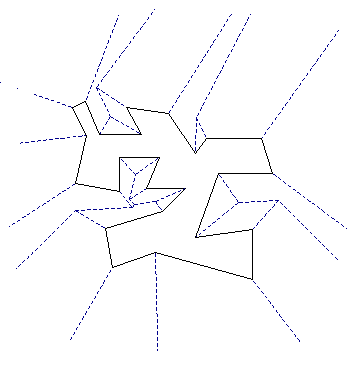
\includegraphics[height=5.6cm, width=5.5cm]{C:/c/fuera.png}%j		

\end{figure}


\column{5cm}

\begin{block}{}
\begin{itemize}
	\item<1-| alert@+>Existencia de caras abiertas.
	\item<2-| alert@+>\'Arboles que no se mezclan .
	\item<3-| alert@+>$|$LCA$|>1$.
\end{itemize}\end{block}
\end{columns}
\transboxin[duration=0.4]
\end{frame}

\subsection{An\'alisis}


\begin{frame}
\frametitle{An\'alisis}
\begin{block}{Definici\'on}
\textcolor{violet}{\'Arbol reflexivo}: \'arbol que tiene un arco reflexivo conectado a su ra\'iz.
\end{block}
\pause
\begin{block}{Presupuesto}
\emph{Una mezcla de corte s\'olo es inducida por un arbol reflexivo. }
\end{block}
\transboxout[duration=0.4]
\end{frame}

\begin{frame}
\frametitle{An\'alisis}
\begin{itemize}
	\item<1-| alert@1>Complejidad espacial $O(n)$
	\item<2->Tiempo de ejecuci\'on para pol\'igonos convexos seg\'un el caso 
	\begin{enumerate}
	\item<3-| alert@3> Construcci\'on de $S(P)$ hacia el exterior de $P$ $O(n)$
	\item<4-| alert@4> Construcci\'on de $S(P)$ hacia el interior de $P$ $O(n\log n)$ (complejidad presupuesta)
	\end{enumerate}
	\item<5-| alert@5>Para pol\'igonos no convexos se est\'a analizando un costo amortizado	del algoritmo. 
\end{itemize}
\transboxout[duration=0.4]
\end{frame}
%%%%%%%%%%%%%%%%%%%%%%%%%%%%%%%%%%%%%%%%%%%%%%%%%%%%
\section{Las paralelas}
\subsection{Relaci\'on con las caras de S(P)}
%%%%%%%%%%%%%%%%%%%%%%%%%%%%%%%%%%%%%%%%%%%%%%%%
\begin{frame}
\frametitle{Relaci\'{o}n entre las caras del esqueleto y las aristas de la
poligonal resultante.}
\begin{itemize}
	\item<1-| alert@+>Recorrido por las caras de $S(P)$
	\item<2-| alert@+>$p(e)$ recta paralela a la arista $e$ a distancia $d$ 
	\item<3-| alert@+>B\'usqueda de las intersecciones entre $p(e)$ y los arcos que conforman la cara que involucra a $e$
	%\item<4->Cara abierta representa la cara formada por los arcos de la ladera de dos \'arboles en LCA adtacentes
\end{itemize}
\transsplithorizontalout[duration=0.4]
\end{frame}

\begin{frame}
\frametitle{Contrucci\'on de la poligonal resultante a partir del esqueleto recto}
\begin{block}{}
Cara abierta: representa la cara formada por los arcos de la laderas cercanas de dos \'arboles en la LCA adyacentes.
\end{block}
\begin{figure}
	\centering
		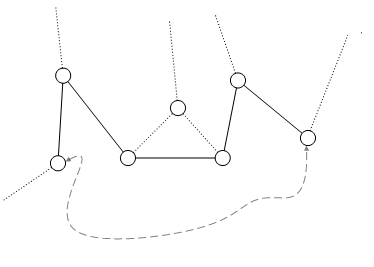
\includegraphics[height=4.5cm, width=6cm]{C:/c/cara.png}%j	 	

\end{figure}
\transdissolve[duration=0.4]
\end{frame}

\begin{frame}
\frametitle{$S(P)$ en una vista arb\'orea}

\begin{columns}[6cm]
\column{5cm}

\begin{figure}
	\centering
		\includegraphics[height=4cm, width=5cm]{C:/c/ar.png}%j	 	
%		\includegraphics<2>[height=5.2cm, width=11cm]{C:/c/arbol1.png}%j	 	
\end{figure}

\column{5cm}

\begin{figure}
	\centering
		\includegraphics<1>[height=4cm, width=5cm]{C:/c/ar2.png}%j	 	
		\includegraphics<2>[height=4cm, width=5cm]{C:/c/arbol1.png}%j	 	
\end{figure}

\end{columns}
\transboxin<1>[duration=0.4]
\end{frame}

\begin{frame}
\frametitle{An\'alisis}
\begin{itemize}
	\item<1->Complejidad espacial $O(n)$ ya que se almacena el conjunto resultado a medida en que se va obteniendo
	\item<2->Tiempo de ejecuci\'on determinado por el recorrido por las caras de $S(P)$. $O(n)$
	\begin{itemize}
	\item<3-> Se pasa sobre cada  arco arco dos veces 
	\item<4-> N\'umero de arcos acotado por $2n-3$
	\end{itemize}	
\end{itemize}
\transboxout[duration=0.4]
\end{frame}

\section{Conclusiones}

\begin{frame}
\frametitle{Conclusiones}
\begin{block}{}
\begin{enumerate}

\item<1-| alert@1> Presentaci\'on de un algoritmo para el c\'omputo del conjunto de pol\'igonos resultante del crecimiento o decrecimiento de un pol\'igono mediante paralelas.

\item<2-| alert@2>  Evidencia de la complejidad de una soluci\'on directa a este problema.
\item<3-| alert@3> Detalles de implementaci\'on del algoritmo de construcci\'on del esqueleto recto de un pol\'igono simple.

\item<4-| alert@4> Algoritmo para la obtenci\'on del conjunto resultado a partir de dicho esqueleto.  

\end{enumerate}
\end{block}
\transsplithorizontalout[duration=0.4]
\end{frame}	

\section{Preguntas}
\begin{frame}
\frametitle{Preguntas}
\begin{itemize}

\item<1-> En el trabajo se define el esqueleto recto como: el rastro que dejan los v\'ertices del pol\'igono inicial cuando este se va encogiendo o ensanchando, movi\'endose cada una de sus aristas a una misma velocidad. Esta definici\'on contiene la soluci\'on del problema que intenta resolver la tesis. Entonces; \textquestiondown No podr\'ia pensarse en un algoritmo que, dando una cantidad de pasos $x$ del m\'etodo para calcular el esqueleto recto del pol\'igono, encuentre la soluci\'on de este problema, sin necesidad de completar el esqueleto y sin tener que realizar el algoritmo siguiente de calcular el pol\'igono buscado a partir de las caras obtenidas con el esqueleto? 

\end{itemize}
\transdissolve[duration=0.4]
\end{frame}

\begin{frame}
\frametitle{Preguntas}
\begin{itemize}

\item<1-> \textquestiondown C\'omo son tratados los errores num\'ericos en el trabajo y que consecuencias podr\'ian tener en la aplicaci\'on del algoritmo dado? \textquestiondown Podr\'ian llevar a una secuencia incorrecta de eventos que creen una soluci\'on no deseada? 

\end{itemize}
\transdissolve[duration=0.4]
\end{frame}

\begin{frame}
\frametitle{Respuestas}
\begin{block}{Respuesta 1}
\begin{itemize}
\item<1-| alert@+> V\'ertices reflexivos
\item<2-| alert@+> Mezcla de corte

\end{itemize}
\end{block}

\begin{block}{Respuesta 2}
\begin{itemize}
\item<3-| alert@+> Aproximaci\'on con epsilon 
\item<4-| alert@+> Eventos m\'ultiples
\item<5-| alert@+> Conocimiento previo

\end{itemize}
\end{block}
\transboxin[duration=0.2]
\end{frame}

\section{Ap\'endice}

\begin{frame}
\frametitle{Ap\'endice}
\end{frame}


\subsection{Demostraciones}


\againframe<beamer| beamer:2>{pspacecomplete}
\againframe<beamer| beamer:2>{pspacecomplete1}
\againframe<beamer| beamer:2>{pspacecomplete2}





\end{document}
